\section{Results and discussion}
\subsection{Effect of operating temperature on water flow rate outflow from air side}

Figure \ref{fig:fig4a} shows the change in the water flow out of the air side at different working temperatures. As can be seen from the figure \ref{fig:fig5a}, as the temperature rises, the water content in the air side exhaust gas generally shows an upward trend. The higher the temperature, the higher the saturation vapor pressure of the fuel cell. Under the same water content, the relative humidity will decrease at this time, which is equivalent to the generation of less liquid water inside the fuel cell, and the ability of the gas to carry water is improved. This change applies to both the air side and the hydrogen side, which is shown in figure \ref{fig:fig4b} and figure \ref{fig:fig4c}. Therefore, under the same other conditions, the water flow out of the fuel cell stack by the air increases with the increase in temperature, and more liquid water is collected by the air side exhaust gas collection device.
\par
It is worth noting that when the load current is 120A, the impact of the working temperature on the water flow of the air side is slightly different under different metering ratios. As the air metering ratio increases, the growth rate of the water flow on the air side gradually decreases. This is because at a small current density, the fuel cell produces less water due to the electrochemical reaction, and at the same time, the high-speed high-temperature reaction gas has a strong ability to carry water, and the water produced by the fuel cell has been completely carried out by the reaction gas. Therefore, even if the air metering ratio increases, the reaction gas cannot carry out more water. For the working conditions of low working temperature and large load current, the ability of the reaction gas to carry water is low or the fuel cell produces more water, so there is still some water vapor or liquid water remaining in the system. At this time, if the air flow is increased, the water flow out of the system will also increase accordingly.

\subfile{Airside_Waterflow_figure_1.tex}
\par
Fig \ref{fig:fig5a} shows that as the temperature rises, the water content in the hydrogen side exhaust gas generally shows a downward trend, and even at 120A/70$^{\circ}C$, the water content in the hydrogen side exhaust gas is 0, the same result appears in 210A(fig \ref{fig:fig5b}) and 300A(fig \ref{fig:fig5c}). There are mainly two reasons for this phenomenon.  First, according to the principle of proton exchange membrane fuel cell reaction, the reaction product water is generated at the cathode (that is, the air side), and the fuel used by the fuel cell system is 99.99\% pure hydrogen. Therefore, the water inside the hydrogen side is mainly the water that migrates from the air side to the hydrogen side under the action of concentration diffusion and pressure diffusion. Since the hydrogen-air pressure difference is basically consistent (20kpa) during the experiment, the influence of pressure on water migration can be ignored when comparing. Second, the exhaust gas collected on the anode side needs to first pass through the water separator built into the fuel cell system to separate the unreacted hydrogen from the liquid water, and then it can be collected by the exhaust water collection device on the hydrogen side. And at higher working temperatures, the saturation vapor pressure of the gas on the hydrogen side rises, and the content of liquid water decreases relatively. These two factors cause the working temperature to rise and the water content flowing out of the hydrogen side to decrease.

\subfile{Airside_Waterflow_figure_2.tex}

\subsection{Influence of air metering ratio on the water flow out of the cathode and anode}

Compare the water flow out of the air side and the hydrogen side at 120A, 210A, 300A load currents, different coolant inlet temperatures, and different air metering ratios, as shown in Fig \ref{fig:fig6a}. Similar to the impact of working temperature on the water flow out of the air side, under the same load current, the higher the air metering ratio, the more water is carried out of the stack by the unreacted air, which also applies to load current of 210A(fig \ref{fig:fig6b}) and 300A(fig \ref{fig:fig6c}). It should be noted that this growth is not unlimited. After reaching a certain air metering ratio, the growth of the water content in the air side exhaust gas slows down, especially when the load current is small and the working temperature is high. This is because at this time, the water produced by the electrochemical reaction of the fuel cell has been completely carried out of the fuel cell by high-temperature high-speed air. At this time, even if the air metering ratio continues to increase, the water content of the exhaust gas will not continue to increase.
\subfile{Airside_Waterflow_figure_grouped_by_temperature.tex}
\par
For the hydrogen side, similarly, as the air metering ratio increases, the water flow out of the hydrogen side basically continues to decrease. After the above analysis, as the air metering ratio increases, the water stored in the cathode will be taken out of the stack by the high-speed airflow, and the water flow diffused to the hydrogen side through concentration difference becomes less, so relatively speaking, the water collected on the hydrogen side will become less. However, the degree of decline is different. Under low temperature (120A/60$^{\circ}C$, 210A/60$^{\circ}C$, and 300A/63$^{\circ}C$), they all show a relatively gentle decline. As the temperature rises, the water flow out of the hydrogen side is also gradually affected by the air metering ratio.

\subfile{Hydroside_Waterflow_figure_grouped_by_temperature.tex}

\subsection{Effects of operating temperature and air metering ratio on internal water content of fuel cell system}
According to the working principle of the fuel cell, during the reaction process, water mainly comes from the electrochemical reaction and the water vapor that enters the fuel cell with the reaction gas. Then, a part of the water is discharged from the fuel cell with the exhaust gas after the reaction, and another part of the water stays inside the fuel cell. In this article, the change rate of the water remaining in the fuel cell will be used as the research object to evaluate the water content status inside the fuel cell.
\begin{equation}
	\label{eq9}
	{\frac{d m_{w,s t k}}{d t}}=Q_{w,i n,s y s}+Q_{w,g e n}-Q_{w,o u t,c a}-Q_{w,o u t,a n}
\end{equation}
In formula \ref{eq9}, $m_(w,stk)$ is the water content inside the fuel cell, in g, $Q_(w,in,sys)$ is the water flow rate entering the fuel cell system, in (g/s), $Q_(w,gen)$ represents the water flow rate generated by the electrochemical reaction, in (g/s), $Q_(w,out,ca)$ represents the water flow rate flowing out of the system from the cathode, in (g/s), $Q_(w,out,an)$ represents the water flow rate flowing out of the system from the anode, in (g/s).
\par
Although during the reaction process, under the effects of concentration diffusion and electro-osmotic drag, water at the cathode will migrate to the anode. However, the research object of the water balance method is the entire fuel cell, so the internal water migration process will not have an impact.
\par
Using the method described above, the rate of change of the water content inside the fuel cell system under different load currents, working temperatures, and air metering ratios can be calculated. In the process of making the graph, to maintain the integrity of the graph. We use (Load current/Temperature/Coefficient) as the format of test environment description. The data of (210A/55$^{\circ}C$/1.8 ) and (210A/55$^{\circ}C$/2.0) are replaced with (210A/55$^{\circ}C$/2.2) test's data. The obtained results are compared as shown in Fig \ref{fig:fig8a}, Fig \ref{fig8b} and Fig \ref{fig:fig8c}, where positive values indicate an increase in water content (represented in blue), and negative values indicate a decrease in water content (represented in red). For the convenience of subsequent discussions, the blue part is defined as flooding, the red part is defined as drying, and the green part is defined as the normal state.

\begin{figure}
	\label{fig:figure8}

		\label{fig:fig8a}
		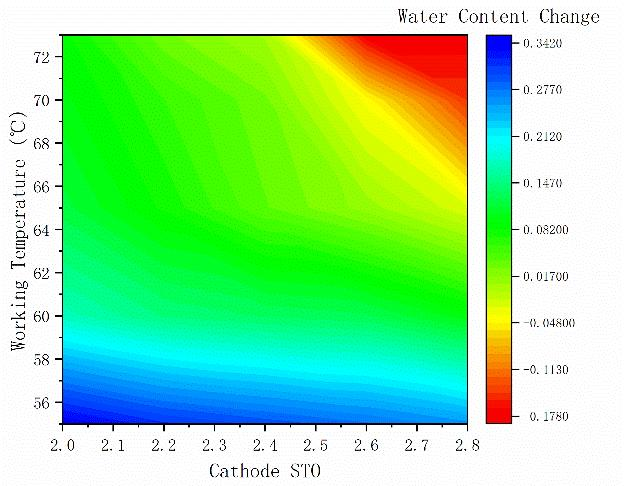
\includegraphics[width=0.5\textwidth]{Research_pictures/fig8a.jpg}
		\label{fig:fig8b}
		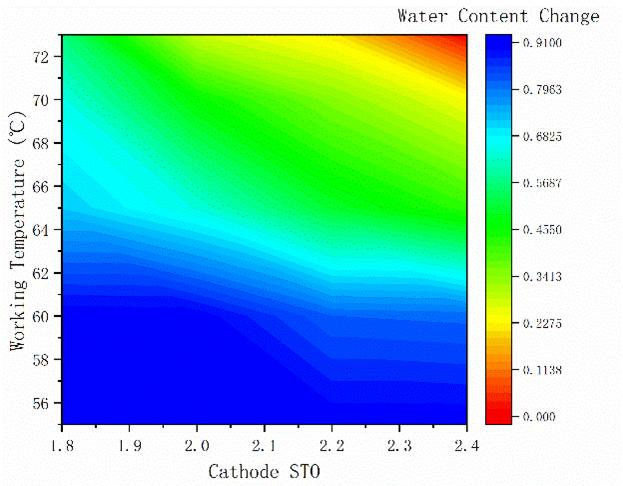
\includegraphics[width=0.5\textwidth]{Research_pictures/fig8b.jpg}
		\label{fig:fig8c}
		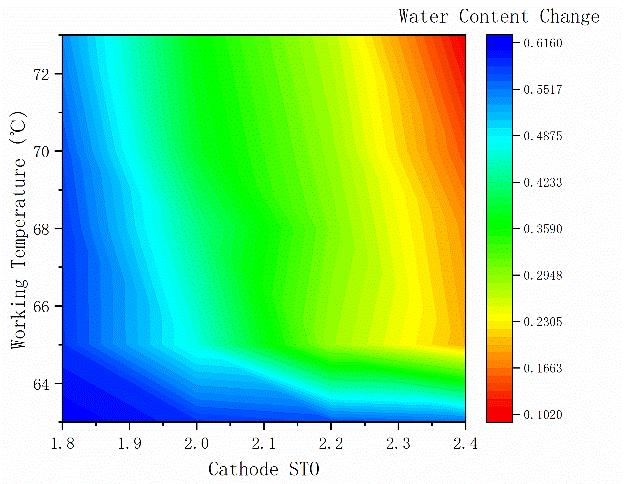
\includegraphics[width=0.5\textwidth]{Research_pictures/fig8c.jpg}
	\caption{Comparison chart of internal water content of fuel cell system under different conditions (a:120A; b:210A; c:300A)}
\end{figure}

As can be seen from Fig \ref{fig:figure8}, under the same load current, as the working temperature increases and the air metering ratio increases, the rate of change of the water content inside the fuel cell system gradually decreases. When it is 120A/73$^{\circ}C$/2.8, 210A/73$^{\circ}C$/2.4, 300A/73$^{\circ}C$/2.4, the rate of change of the water content inside the fuel cell system reaches the minimum value under this load current. However, the degree of influence of the working temperature and the air metering ratio on the rate of change of the water content inside the fuel cell system is slightly different. When the load current is 120A and 210A, too low working temperature is more likely to cause flooding than too low air metering ratio. For example, at 120A, when the working temperature is 55$^{\circ}C$, even if the air metering ratio reaches 2.8, the fuel cell system is still in a relatively flooded state; and when the working temperature is 73$^{\circ}C$, even if the air metering ratio is only 2.0, the fuel cell system is in a normal state. In a dry state, the degree of influence of working temperature and air metering ratio is not much different. However, when the load current is 310A, the trend is the opposite. Too low working temperature and too low air metering ratio will cause flooding, and too high air metering ratio is more likely to cause drying than too high working temperature.

\par
Furthermore, this paper uses the method of linear regression to analyze the impact of working temperature and air metering ratio on the water content inside the fuel cell system. Before this, the data needs to be standardized. This paper uses the Z-score normalization method, which is
$$x^{*}=x-\mu\sigma$$

\par
Table \ref{tab:RegressionAnalysis} shows the result of analysis:
\begin{table}
	\centering
	\begin{center}
		\caption{Regression analysis under different load current}
		\label{tab:RegressionAnalysis}
		\begin{tabular}{l|l|l}
			\hline
			\textbf{Load current(A)} & \textbf{\makecell{Temperature ratio\\regression coefficient}} & \textbf{\makecell{Air metering\\ratio regression coefficient}} \\
			\hline
			120                       & -0.8469                                           & -0.4145                                            \\
			210                       & -0.9341                                           & -0.4347                                            \\
			300                       & -0.4637                                           & -0.7618                                            \\
			\hline
		\end{tabular}
	\end{center}
\end{table}
Similar to the phenomenon described above, the impact of the working temperature is more significant when the load current is 120A and 210A; while the impact of the air metering ratio is more significant when the load current is 300A. The reason for this phenomenon may be: the air metering ratio is related to the load current. Under different load currents, the air metering ratio changes the same magnitude, but the change in air flow is different. Since the fuel cell system needs to rely on high-speed high-temperature gas to carry the water out, the higher the load current, the more significant the impact of the air metering ratio.
\par
Therefore, to maintain the long-term stable operation of the fuel cell system, appropriate operating conditions need to be selected. The following principles should be considered when choosing:
\begin{itemize}
	\item The fuel cell system should be in a normal state under this condition;
	\item In the actual operation process, there are certain fluctuations in the working temperature and air metering ratio. The fluctuation range of the working temperature is about $\pm2^{\circ}C$, and the fluctuation range of the air metering ratio is about$\pm0.1$, so the selected conditions should make the points within the fluctuation range in a normal state;
	\item A larger air metering ratio and a lower working temperature will cause additional consumption of the auxiliary system, so try to choose working conditions with a low air metering ratio and a high working temperature.
\end{itemize}
As shown in Fig \ref{fig:figure9}, 120A/67$^{\circ}C$/2.15, 210A/68$^{\circ}C$/2.15, 300A/70$^{\circ}C$/2.05 are selected as the appropriate operating conditions under each load current.
\begin{figure}
	\label{fig:figure9}
	% \subfigure[]{
		\label{fig:fig9a}
		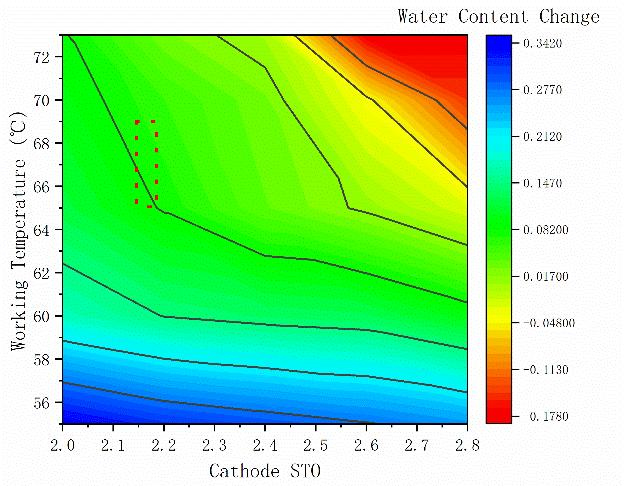
\includegraphics[width=0.5\textwidth]{Research_pictures/fig9a.jpg}
	% }
	% \subfigure[]{
		\label{fig:fig9b}
		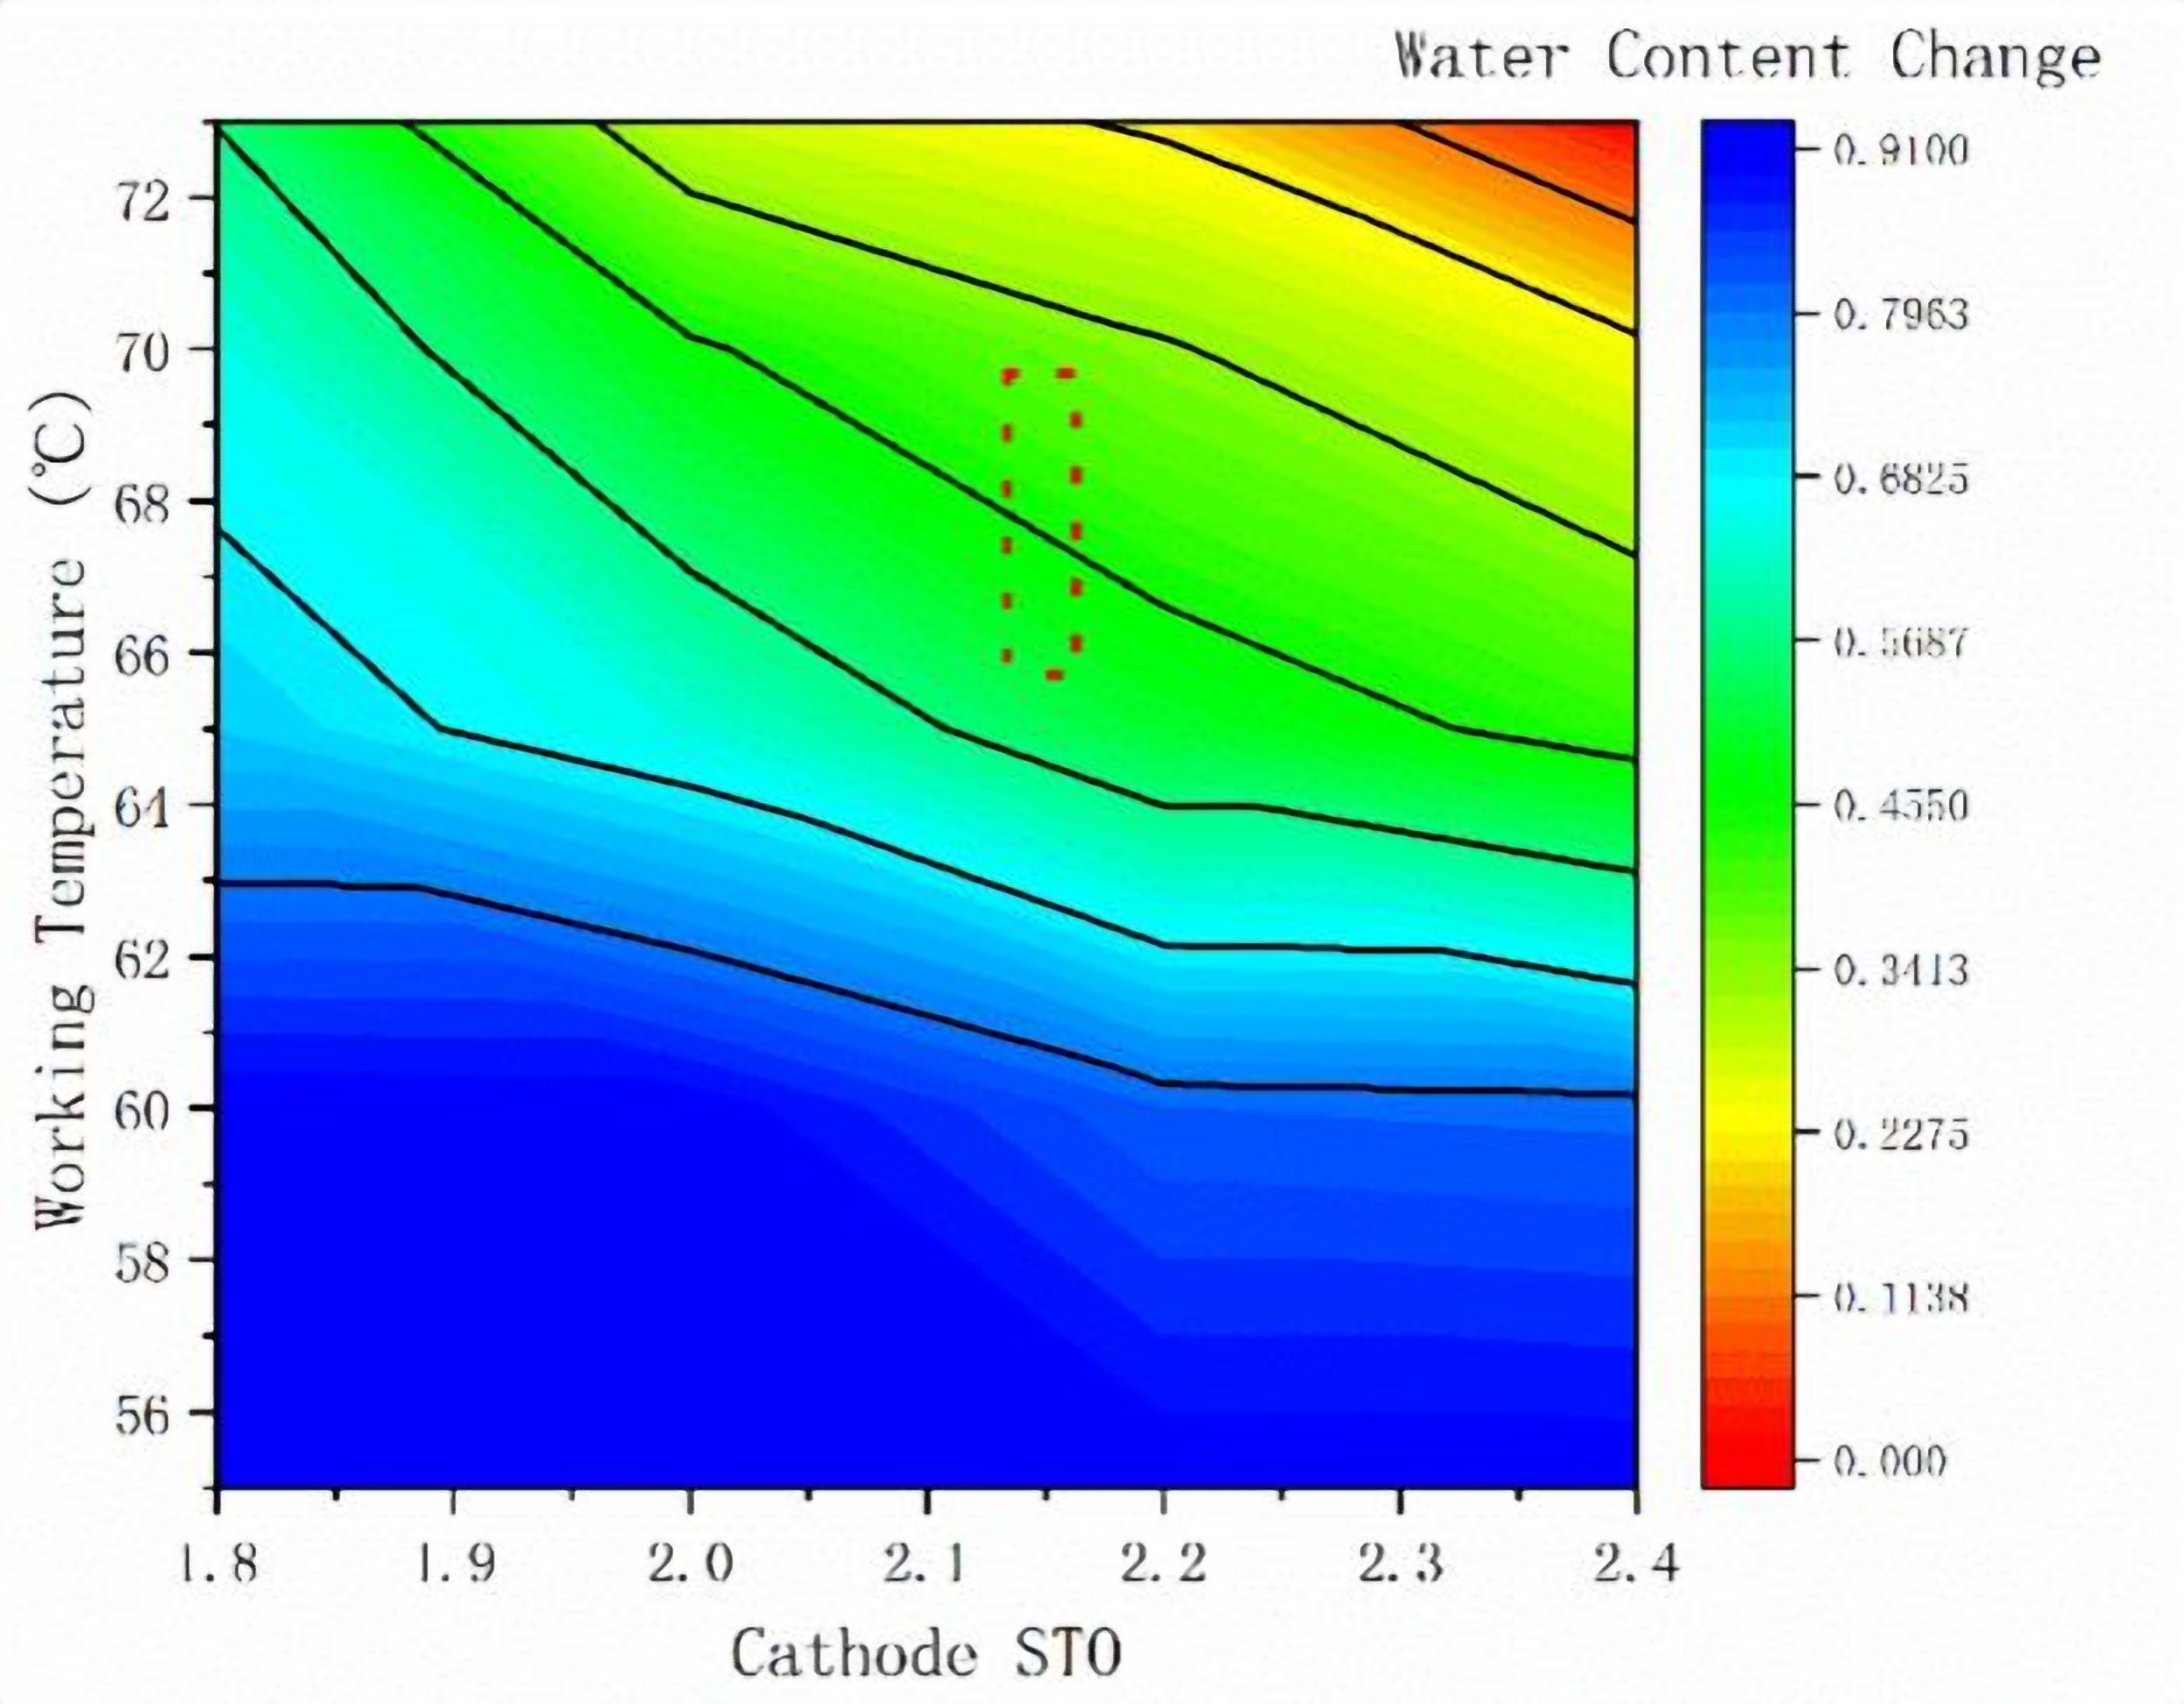
\includegraphics[width=0.5\textwidth]{Research_pictures/fig9b.jpg}
	% }
	% \subfigure[]{
		\label{fig:fig9c}
		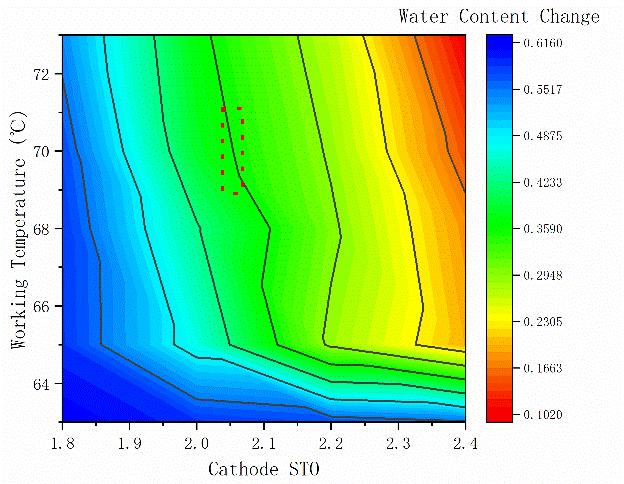
\includegraphics[width=0.5\textwidth]{Research_pictures/fig9c.jpg}
	% }
	\caption{Selection of fuel cell OS operating environment (Working environment surrounded by dots, a:120A; b:210A; c:300A)}
\end{figure}
Next, compare the rate of change of the water content inside the fuel cell system under different load currents.

\begin{table}
	\centering
	\begin{center}
		\caption{Statistical table of the change rate of internal water content of different load currents}
		\label{tab:StatisticalTable}
		\begin{tabular}{l|c|c|c|c|r}
			\hline
			\textbf{Load current(A)} & \textbf{maximum} & \textbf{minimum} & \textbf{range} & \textbf{average} & \textbf{variance} \\
			\hline
			120                       & 0.342            & -0.177           & 0.519          & 0.086            & 0.019             \\
			210                       & 0.909            & 0.009            & 0.900          & 0.562            & 0.067             \\
			300                       & 0.615            & 0.103            & 0.512          & 0.402            & 0.028             \\
			\hline
		\end{tabular}
	\end{center}
\end{table}
From Table \ref{tab:StatisticalTable}, it can be seen that as the load current increases, the rate of change of the water content inside the fuel cell system increases to some extent, but the increase is not large. This may be because the higher the load current of the fuel cell, the more water flow is generated, so the water accumulated inside correspondingly increases. In addition, it was found that when the load current is 210A, the range is larger compared to 120A and 300A. Correspondingly, the fuel cell system cannot operate stably under the conditions of 210A/55$^{\circ}C$/1.6 and 210A/55$^{\circ}C$/1.8. This further reflects the connection between the rate of change of the internal water content of the fuel cell system and the water content fault.
\par
However, the above calculation method can only calculate the absolute value of the water content inside the fuel cell system. The output performance of the fuel cell in actual operation is related to the working temperature, intake pressure, and air metering ratio. To find the most suitable working conditions under each load current, it is necessary to establish a fuel cell stack model, and study the correlation between the difference between the actual output and theoretical output of the fuel cell stack under different conditions and the absolute value of the water content inside the fuel cell system.
